\chapter{Wykorzystane narzędzia, dokumentacja i kody pakietu $\mathcal{R}$ użyte w pracy}\label{docCoxSGD}
\section{Model proporcjonalnych hazardów Coxa}\label{coxKody123}

\begin{Shaded}
\begin{Highlighting}[]
\NormalTok{checkArguments <-}\StringTok{ }\NormalTok{function(formula, data, learningRates,}
                             \NormalTok{beta_0, epsilon) \{}
  \KeywordTok{assert_that}\NormalTok{(}\KeywordTok{is.list}\NormalTok{(data) &}\StringTok{ }\KeywordTok{length}\NormalTok{(data) >}\StringTok{ }\DecValTok{0}\NormalTok{)}
  \KeywordTok{assert_that}\NormalTok{(}\KeywordTok{length}\NormalTok{(}\KeywordTok{unique}\NormalTok{(}\KeywordTok{unlist}\NormalTok{(}\KeywordTok{lapply}\NormalTok{(data, ncol)))) ==}\StringTok{ }\DecValTok{1}\NormalTok{)}
  \CommentTok{# + check names and types for every variables}
  \KeywordTok{assert_that}\NormalTok{(}\KeywordTok{is.function}\NormalTok{(learningRates))}
  \KeywordTok{assert_that}\NormalTok{(}\KeywordTok{is.numeric}\NormalTok{(epsilon))}
  \KeywordTok{assert_that}\NormalTok{(}\KeywordTok{is.numeric}\NormalTok{(beta_0))}
  
    \CommentTok{# check length of the start parameter}
  \NormalTok{if (}\KeywordTok{length}\NormalTok{(beta_0) ==}\StringTok{ }\DecValTok{1}\NormalTok{) \{}
    \NormalTok{beta_0 <-}\StringTok{ }\KeywordTok{rep}\NormalTok{(beta_0, }\KeywordTok{as.character}\NormalTok{(formula)[}\DecValTok{3}\NormalTok{] %>%}
\StringTok{                    }\KeywordTok{strsplit}\NormalTok{(}\StringTok{"}\CharTok{\textbackslash{}\textbackslash{}}\StringTok{+"}\NormalTok{) %>%}
\StringTok{                    }\NormalTok{unlist %>%}
\StringTok{                    }\NormalTok{length)}
  \NormalTok{\}}
  \KeywordTok{return}\NormalTok{(beta_0)}
\NormalTok{\}}
\end{Highlighting}
\end{Shaded}


\begin{Shaded}
\begin{Highlighting}[]
\NormalTok{prepareBatch <-}\StringTok{ }\NormalTok{function(formula, data) \{}
  \CommentTok{# Parameter identification as in  `survival::coxph()`.}
  \NormalTok{Call <-}\StringTok{ }\KeywordTok{match.call}\NormalTok{()}
  \NormalTok{indx <-}\StringTok{ }\KeywordTok{match}\NormalTok{(}\KeywordTok{c}\NormalTok{(}\StringTok{"formula"}\NormalTok{, }\StringTok{"data"}\NormalTok{),}
                \KeywordTok{names}\NormalTok{(Call), }\DataTypeTok{nomatch =} \DecValTok{0}\NormalTok{)}
  \NormalTok{if (indx[}\DecValTok{1}\NormalTok{] ==}\StringTok{ }\DecValTok{0}\NormalTok{) }
      \KeywordTok{stop}\NormalTok{(}\StringTok{"A formula argument is required"}\NormalTok{)}
  \NormalTok{temp <-}\StringTok{ }\NormalTok{Call[}\KeywordTok{c}\NormalTok{(}\DecValTok{1}\NormalTok{, indx)]}
  \NormalTok{temp[[}\DecValTok{1}\NormalTok{]] <-}\StringTok{ }\KeywordTok{as.name}\NormalTok{(}\StringTok{"model.frame"}\NormalTok{)}
  
  \NormalTok{mf <-}\StringTok{ }\KeywordTok{eval}\NormalTok{(temp, }\KeywordTok{parent.frame}\NormalTok{())}
  \NormalTok{Y <-}\StringTok{ }\KeywordTok{model.extract}\NormalTok{(mf, }\StringTok{"response"}\NormalTok{)}
  
  \NormalTok{if (!}\KeywordTok{inherits}\NormalTok{(Y, }\StringTok{"Surv"}\NormalTok{)) }
      \KeywordTok{stop}\NormalTok{(}\StringTok{"Response must be a survival object"}\NormalTok{)}
  \NormalTok{type <-}\StringTok{ }\KeywordTok{attr}\NormalTok{(Y, }\StringTok{"type"}\NormalTok{)}
  
  \NormalTok{if (type !=}\StringTok{ "right"} \NormalTok{&&}\StringTok{ }\NormalTok{type !=}\StringTok{ "counting"}\NormalTok{) }
      \KeywordTok{stop}\NormalTok{(}\KeywordTok{paste}\NormalTok{(}\StringTok{"Cox model doesn't support }\CharTok{\textbackslash{}"}\StringTok{"}\NormalTok{, type, }\StringTok{"}\CharTok{\textbackslash{}"}\StringTok{ survival data"}\NormalTok{, }
          \DataTypeTok{sep =} \StringTok{""}\NormalTok{))}
  
  \CommentTok{# collect times, status, variables and reorder samples }
  \CommentTok{# to make the algorithm more clear to read and track}
  \KeywordTok{cbind}\NormalTok{(}\DataTypeTok{event =} \KeywordTok{unclass}\NormalTok{(Y)[,}\DecValTok{2}\NormalTok{], }\CommentTok{# 1 indicates event, 0 indicates cens}
        \DataTypeTok{times =} \KeywordTok{unclass}\NormalTok{(Y)[,}\DecValTok{1}\NormalTok{],}
        \NormalTok{mf[, -}\DecValTok{1}\NormalTok{]) %>%}
\StringTok{    }\KeywordTok{arrange}\NormalTok{(times) }
\NormalTok{\}}
\end{Highlighting}
\end{Shaded}
\begin{Shaded}
\begin{Highlighting}[]
\NormalTok{full_cox_loglik <-}\StringTok{ }\NormalTok{function(beta1, beta2, x1, x2, censored)\{}
  \KeywordTok{sum}\NormalTok{(}\KeywordTok{rev}\NormalTok{(censored)*(beta1*}\KeywordTok{rev}\NormalTok{(x1) +}\StringTok{ }\NormalTok{beta2*}\KeywordTok{rev}\NormalTok{(x2) -}
\StringTok{                       }\KeywordTok{log}\NormalTok{(}\KeywordTok{cumsum}\NormalTok{(}\KeywordTok{exp}\NormalTok{(beta1*}\KeywordTok{rev}\NormalTok{(x1) +}\StringTok{ }\NormalTok{beta2*}\KeywordTok{rev}\NormalTok{(x2))))))}
\NormalTok{\}}


\NormalTok{calculate_outer_cox <-}\StringTok{ }\NormalTok{function(x1, x2, censored)\{}
  \NormalTok{## contours}
  \NormalTok{outer_res <-}\StringTok{ }\KeywordTok{outer}\NormalTok{(}\KeywordTok{seq}\NormalTok{(-}\DecValTok{1}\NormalTok{,}\DecValTok{3}\NormalTok{, }\DataTypeTok{length =} \DecValTok{100}\NormalTok{),}
           \KeywordTok{seq}\NormalTok{(}\DecValTok{0}\NormalTok{,}\DecValTok{4}\NormalTok{, }\DataTypeTok{length =} \DecValTok{100}\NormalTok{),}
           \KeywordTok{Vectorize}\NormalTok{( function(beta1,beta2)\{}
             \KeywordTok{full_cox_loglik}\NormalTok{(beta1, beta2, }\DataTypeTok{x1 =} \NormalTok{x1, }\DataTypeTok{x2 =} \NormalTok{x2, }\DataTypeTok{censored =} \NormalTok{censored)}
           \NormalTok{\} )}
  \NormalTok{)}
  \NormalTok{outer_res_melted <-}\StringTok{ }\KeywordTok{melt}\NormalTok{(outer_res)}
  \NormalTok{outer_res_melted$Var1 <-}\StringTok{ }\KeywordTok{as.factor}\NormalTok{(outer_res_melted$Var1)}
  \KeywordTok{levels}\NormalTok{(outer_res_melted$Var1) <-}\StringTok{ }\KeywordTok{as.character}\NormalTok{(}\KeywordTok{seq}\NormalTok{(-}\DecValTok{1}\NormalTok{,}\DecValTok{3}\NormalTok{, }\DataTypeTok{length =} \DecValTok{100}\NormalTok{))}
  \NormalTok{outer_res_melted$Var2 <-}\StringTok{ }\KeywordTok{as.factor}\NormalTok{(outer_res_melted$Var2)}
  \KeywordTok{levels}\NormalTok{(outer_res_melted$Var2) <-}\StringTok{ }\KeywordTok{as.character}\NormalTok{(}\KeywordTok{seq}\NormalTok{(}\DecValTok{0}\NormalTok{,}\DecValTok{4}\NormalTok{, }\DataTypeTok{length =} \DecValTok{100}\NormalTok{))}
  \NormalTok{outer_res_melted$Var1 <-}\StringTok{ }\KeywordTok{as.numeric}\NormalTok{(}\KeywordTok{as.character}\NormalTok{(outer_res_melted$Var1))}
  \NormalTok{outer_res_melted$Var2 <-}\StringTok{ }\KeywordTok{as.numeric}\NormalTok{(}\KeywordTok{as.character}\NormalTok{(outer_res_melted$Var2))}
  \KeywordTok{return}\NormalTok{(outer_res_melted)}
\NormalTok{\}}
\NormalTok{simulateCoxSGD <-}\StringTok{ }\NormalTok{function(}\DataTypeTok{dCox =} \NormalTok{dCox, }\DataTypeTok{learningRates =} \NormalTok{function(x)\{}\DecValTok{1}\NormalTok{/x\},}
                      \DataTypeTok{epsilon =} \FloatTok{1e-03}\NormalTok{, }\DataTypeTok{beta_0 =} \KeywordTok{c}\NormalTok{(}\DecValTok{0}\NormalTok{,}\DecValTok{0}\NormalTok{), }\DataTypeTok{max.iter =} \DecValTok{100}\NormalTok{)\{}

  \KeywordTok{sample}\NormalTok{(}\DecValTok{1}\NormalTok{:}\DecValTok{90}\NormalTok{, }\DataTypeTok{size =} \DecValTok{10}\NormalTok{^}\DecValTok{4}\NormalTok{, }\DataTypeTok{replace =} \OtherTok{TRUE}\NormalTok{) ->}\StringTok{ }\NormalTok{group}
  \KeywordTok{split}\NormalTok{(dCox, group) ->}\StringTok{ }\NormalTok{dCox_splitted}
  \KeywordTok{coxphSGD}\NormalTok{(}\KeywordTok{Surv}\NormalTok{(time, status)~x}\FloatTok{.1}\NormalTok{+x}\FloatTok{.2}\NormalTok{, }\DataTypeTok{data =} \NormalTok{dCox_splitted,}
           \DataTypeTok{epsilon =} \NormalTok{epsilon, }\DataTypeTok{learningRates =} \NormalTok{learningRates, }
           \DataTypeTok{beta_0 =} \NormalTok{beta_0, }\DataTypeTok{max.iter =} \NormalTok{max.iter*}\DecValTok{90}\NormalTok{) ->}\StringTok{ }\NormalTok{estimates}

  \KeywordTok{sample}\NormalTok{(}\DecValTok{1}\NormalTok{:}\DecValTok{60}\NormalTok{, }\DataTypeTok{size =} \DecValTok{10}\NormalTok{^}\DecValTok{4}\NormalTok{, }\DataTypeTok{replace =} \OtherTok{TRUE}\NormalTok{) ->}\StringTok{ }\NormalTok{group}
  \KeywordTok{split}\NormalTok{(dCox, group) ->}\StringTok{ }\NormalTok{dCox_splitted}
  \KeywordTok{coxphSGD}\NormalTok{(}\KeywordTok{Surv}\NormalTok{(time, status)~x}\FloatTok{.1}\NormalTok{+x}\FloatTok{.2}\NormalTok{, }\DataTypeTok{data =} \NormalTok{dCox_splitted,}
           \DataTypeTok{epsilon =} \NormalTok{epsilon, }\DataTypeTok{learningRates =} \NormalTok{learningRates,}
           \DataTypeTok{beta_0 =} \NormalTok{beta_0, }\DataTypeTok{max.iter =} \NormalTok{max.iter*}\DecValTok{60}\NormalTok{) ->}\StringTok{ }\NormalTok{estimates2}

  \KeywordTok{sample}\NormalTok{(}\DecValTok{1}\NormalTok{:}\DecValTok{120}\NormalTok{, }\DataTypeTok{size =} \DecValTok{10}\NormalTok{^}\DecValTok{4}\NormalTok{, }\DataTypeTok{replace =} \OtherTok{TRUE}\NormalTok{) ->}\StringTok{ }\NormalTok{group}
  \KeywordTok{split}\NormalTok{(dCox, group) ->}\StringTok{ }\NormalTok{dCox_splitted}
  \KeywordTok{coxphSGD}\NormalTok{(}\KeywordTok{Surv}\NormalTok{(time, status)~x}\FloatTok{.1}\NormalTok{+x}\FloatTok{.2}\NormalTok{, }\DataTypeTok{data =} \NormalTok{dCox_splitted,}
           \DataTypeTok{epsilon =} \NormalTok{epsilon, }\DataTypeTok{learningRates =} \NormalTok{learningRates,}
           \DataTypeTok{beta_0 =} \NormalTok{beta_0, }\DataTypeTok{max.iter =} \NormalTok{max.iter*}\DecValTok{120}\NormalTok{) ->}\StringTok{ }\NormalTok{estimates3}

  \KeywordTok{sample}\NormalTok{(}\DecValTok{1}\NormalTok{:}\DecValTok{200}\NormalTok{, }\DataTypeTok{size =} \DecValTok{10}\NormalTok{^}\DecValTok{4}\NormalTok{, }\DataTypeTok{replace =} \OtherTok{TRUE}\NormalTok{) ->}\StringTok{ }\NormalTok{group}
  \KeywordTok{split}\NormalTok{(dCox, group) ->}\StringTok{ }\NormalTok{dCox_splitted}
  \KeywordTok{coxphSGD}\NormalTok{(}\KeywordTok{Surv}\NormalTok{(time, status)~x}\FloatTok{.1}\NormalTok{+x}\FloatTok{.2}\NormalTok{, }\DataTypeTok{data =} \NormalTok{dCox_splitted,}
           \DataTypeTok{epsilon =} \NormalTok{epsilon, }\DataTypeTok{learningRates =} \NormalTok{learningRates,}
           \DataTypeTok{beta_0 =} \NormalTok{beta_0, }\DataTypeTok{max.iter =} \NormalTok{max.iter*}\DecValTok{200}\NormalTok{) ->}\StringTok{ }\NormalTok{estimates4}


  \KeywordTok{sample}\NormalTok{(}\DecValTok{1}\NormalTok{:}\DecValTok{30}\NormalTok{, }\DataTypeTok{size =} \DecValTok{10}\NormalTok{^}\DecValTok{4}\NormalTok{, }\DataTypeTok{replace =} \OtherTok{TRUE}\NormalTok{) ->}\StringTok{ }\NormalTok{group}
  \KeywordTok{split}\NormalTok{(dCox, group) ->}\StringTok{ }\NormalTok{dCox_splitted}
  \KeywordTok{coxphSGD}\NormalTok{(}\KeywordTok{Surv}\NormalTok{(time, status)~x}\FloatTok{.1}\NormalTok{+x}\FloatTok{.2}\NormalTok{, }\DataTypeTok{data =} \NormalTok{dCox_splitted,}
           \DataTypeTok{epsilon =} \NormalTok{epsilon, }\DataTypeTok{learningRates =} \NormalTok{learningRates,}
           \DataTypeTok{beta_0 =} \NormalTok{beta_0, }\DataTypeTok{max.iter =} \NormalTok{max.iter*}\DecValTok{30}\NormalTok{) ->}\StringTok{ }\NormalTok{estimates5}


  \KeywordTok{sample}\NormalTok{(}\DecValTok{1}\NormalTok{:}\DecValTok{10}\NormalTok{, }\DataTypeTok{size =} \DecValTok{10}\NormalTok{^}\DecValTok{4}\NormalTok{, }\DataTypeTok{replace =} \OtherTok{TRUE}\NormalTok{) ->}\StringTok{ }\NormalTok{group}
  \KeywordTok{split}\NormalTok{(dCox, group) ->}\StringTok{ }\NormalTok{dCox_splitted}
  \KeywordTok{coxphSGD}\NormalTok{(}\KeywordTok{Surv}\NormalTok{(time, status)~x}\FloatTok{.1}\NormalTok{+x}\FloatTok{.2}\NormalTok{, }\DataTypeTok{data =} \NormalTok{dCox_splitted,}
           \DataTypeTok{epsilon =} \NormalTok{epsilon, }\DataTypeTok{learningRates =} \NormalTok{learningRates,}
           \DataTypeTok{beta_0 =} \NormalTok{beta_0, }\DataTypeTok{max.iter =} \NormalTok{max.iter*}\DecValTok{10}\NormalTok{) ->}\StringTok{ }\NormalTok{estimates6}

  \KeywordTok{t}\NormalTok{(}\KeywordTok{simplify2array}\NormalTok{(estimates$coefficients)) %>%}
\StringTok{    }\KeywordTok{as.data.frame}\NormalTok{() ->}\StringTok{ }\NormalTok{df1}
  \KeywordTok{t}\NormalTok{(}\KeywordTok{simplify2array}\NormalTok{(estimates2$coefficients)) %>%}
\StringTok{    }\KeywordTok{as.data.frame}\NormalTok{() ->}\StringTok{ }\NormalTok{df2}
  \KeywordTok{t}\NormalTok{(}\KeywordTok{simplify2array}\NormalTok{(estimates3$coefficients)) %>%}
\StringTok{    }\KeywordTok{as.data.frame}\NormalTok{() ->}\StringTok{ }\NormalTok{df3}
  \KeywordTok{t}\NormalTok{(}\KeywordTok{simplify2array}\NormalTok{(estimates4$coefficients)) %>%}
\StringTok{    }\KeywordTok{as.data.frame}\NormalTok{() ->}\StringTok{ }\NormalTok{df4}
  \KeywordTok{t}\NormalTok{(}\KeywordTok{simplify2array}\NormalTok{(estimates5$coefficients)) %>%}
\StringTok{    }\KeywordTok{as.data.frame}\NormalTok{() ->}\StringTok{ }\NormalTok{df5}
  \KeywordTok{t}\NormalTok{(}\KeywordTok{simplify2array}\NormalTok{(estimates6$coefficients)) %>%}
\StringTok{    }\KeywordTok{as.data.frame}\NormalTok{() ->}\StringTok{ }\NormalTok{df6}

  \NormalTok{df1 %>%}
\StringTok{    }\KeywordTok{mutate}\NormalTok{(}\DataTypeTok{version =} \KeywordTok{paste}\NormalTok{(}\StringTok{"90 batches,"}\NormalTok{, }\KeywordTok{nrow}\NormalTok{(df1), }\StringTok{" steps"}\NormalTok{)) %>%}
\StringTok{    }\KeywordTok{bind_rows}\NormalTok{(df2 %>%}
\StringTok{                }\KeywordTok{mutate}\NormalTok{(}\DataTypeTok{version =} \KeywordTok{paste}\NormalTok{(}\StringTok{"60 batches,"}\NormalTok{, }\KeywordTok{nrow}\NormalTok{(df2), }\StringTok{" steps"}\NormalTok{))) %>%}
\StringTok{    }\KeywordTok{bind_rows}\NormalTok{(df3 %>%}
\StringTok{                }\KeywordTok{mutate}\NormalTok{(}\DataTypeTok{version =} \KeywordTok{paste}\NormalTok{(}\StringTok{"120 batches,"}\NormalTok{, }\KeywordTok{nrow}\NormalTok{(df3), }\StringTok{" steps"}\NormalTok{))) %>%}
\StringTok{    }\KeywordTok{bind_rows}\NormalTok{(df4 %>%}
\StringTok{                }\KeywordTok{mutate}\NormalTok{(}\DataTypeTok{version =} \KeywordTok{paste}\NormalTok{(}\StringTok{"200 batches,"}\NormalTok{, }\KeywordTok{nrow}\NormalTok{(df4), }\StringTok{" steps"}\NormalTok{))) %>%}
\StringTok{    }\KeywordTok{bind_rows}\NormalTok{(df5 %>%}
\StringTok{                }\KeywordTok{mutate}\NormalTok{(}\DataTypeTok{version =} \KeywordTok{paste}\NormalTok{(}\StringTok{"30 batches,"}\NormalTok{, }\KeywordTok{nrow}\NormalTok{(df5), }\StringTok{" steps"}\NormalTok{))) %>%}
\StringTok{    }\KeywordTok{bind_rows}\NormalTok{(df6 %>%}
\StringTok{                }\KeywordTok{mutate}\NormalTok{(}\DataTypeTok{version =} \KeywordTok{paste}\NormalTok{(}\StringTok{"10 batches,"}\NormalTok{, }\KeywordTok{nrow}\NormalTok{(df6), }\StringTok{" steps"}\NormalTok{))) ->}\StringTok{ }\NormalTok{d2ggplot}

  \KeywordTok{return}\NormalTok{(}\KeywordTok{list}\NormalTok{(}\DataTypeTok{d2ggplot =} \NormalTok{d2ggplot, }\DataTypeTok{est1 =} \NormalTok{estimates, }\DataTypeTok{est2 =} \NormalTok{estimates2,}
              \DataTypeTok{est3 =} \NormalTok{estimates3, }\DataTypeTok{est4 =} \NormalTok{estimates4, }\DataTypeTok{est5 =} \NormalTok{estimates5))}

\NormalTok{\}}
\KeywordTok{simulateCoxSGD}\NormalTok{(dCox, }\DataTypeTok{learningRates =} \NormalTok{function(x)\{}\DecValTok{1}\NormalTok{/(}\DecValTok{100}\NormalTok{*}\KeywordTok{sqrt}\NormalTok{(x))\},}
               \DataTypeTok{max.iter =} \DecValTok{10}\NormalTok{, }\DataTypeTok{epsilon =} \FloatTok{1e-5}\NormalTok{) ->}\StringTok{ }\NormalTok{d2ggplot}
\NormalTok{d2ggplot ->}\StringTok{ }\NormalTok{backpack}
\NormalTok{d2ggplot <-}\StringTok{ }\NormalTok{d2ggplot$d2ggplot}
\NormalTok{beta_0 =}\StringTok{ }\KeywordTok{c}\NormalTok{(}\DecValTok{0}\NormalTok{,}\DecValTok{0}\NormalTok{)}
\NormalTok{solution =}\StringTok{ }\KeywordTok{c}\NormalTok{(}\DecValTok{1}\NormalTok{,}\DecValTok{3}\NormalTok{)}

\KeywordTok{pdf}\NormalTok{(}\DataTypeTok{file =} \StringTok{"b_0_0_iter_10_e-5_100sqrt_878.pdf"}\NormalTok{, }\DataTypeTok{width =} \DecValTok{10}\NormalTok{, }\DataTypeTok{height =} \DecValTok{10}\NormalTok{)}
\KeywordTok{ggplot}\NormalTok{() +}
\StringTok{  }\KeywordTok{stat_contour}\NormalTok{(}\KeywordTok{aes}\NormalTok{(}\DataTypeTok{x=}\NormalTok{outerCox$Var1,}
                   \DataTypeTok{y=}\NormalTok{outerCox$Var2,}
                   \DataTypeTok{z=}\NormalTok{outerCox$value),}
               \DataTypeTok{bins =} \DecValTok{40}\NormalTok{, }\DataTypeTok{alpha =} \FloatTok{0.25}\NormalTok{) +}
\StringTok{  }\KeywordTok{geom_path}\NormalTok{(}\KeywordTok{aes}\NormalTok{(d2ggplot$V1, d2ggplot$V2, }\DataTypeTok{group =} \NormalTok{d2ggplot$version,}
                \DataTypeTok{colour =} \NormalTok{d2ggplot$version), }\DataTypeTok{size =} \DecValTok{1}\NormalTok{) +}
\StringTok{  }\KeywordTok{theme_bw}\NormalTok{(}\DataTypeTok{base_size =} \DecValTok{20}\NormalTok{) +}
\StringTok{  }\KeywordTok{theme}\NormalTok{(}\DataTypeTok{panel.border =} \KeywordTok{element_blank}\NormalTok{(),}
        \DataTypeTok{legend.key =} \KeywordTok{element_blank}\NormalTok{(), }\DataTypeTok{legend.position =} \StringTok{"top"}\NormalTok{) +}
\StringTok{  }\KeywordTok{scale_colour_brewer}\NormalTok{(}\DataTypeTok{palette=}\StringTok{"Dark2"}\NormalTok{, }\DataTypeTok{name =} \StringTok{'Algorithm }\CharTok{\textbackslash{}n}\StringTok{ & Steps'}\NormalTok{) +}
\StringTok{  }\KeywordTok{geom_point}\NormalTok{(}\KeywordTok{aes}\NormalTok{(}\DataTypeTok{x =} \NormalTok{beta_0[}\DecValTok{1}\NormalTok{], }\DataTypeTok{y =} \NormalTok{beta_0[}\DecValTok{2}\NormalTok{]), }\DataTypeTok{col =} \StringTok{"black"}\NormalTok{, }\DataTypeTok{size =} \DecValTok{4}\NormalTok{, }\DataTypeTok{shape =} \DecValTok{17}\NormalTok{) +}
\StringTok{  }\KeywordTok{geom_point}\NormalTok{(}\KeywordTok{aes}\NormalTok{(}\DataTypeTok{x =} \NormalTok{solution[}\DecValTok{1}\NormalTok{], }\DataTypeTok{y =} \NormalTok{solution[}\DecValTok{2}\NormalTok{]), }\DataTypeTok{col =} \StringTok{"black"}\NormalTok{, }\DataTypeTok{size =} \DecValTok{4}\NormalTok{, }\DataTypeTok{shape =} \DecValTok{15}\NormalTok{) +}
\StringTok{  }\KeywordTok{xlab}\NormalTok{(}\StringTok{"X1"}\NormalTok{) +}\StringTok{ }\KeywordTok{ylab}\NormalTok{(}\StringTok{"X2"}\NormalTok{) +}
\StringTok{  }\KeywordTok{guides}\NormalTok{(}\DataTypeTok{col =} \KeywordTok{guide_legend}\NormalTok{(}\DataTypeTok{ncol =} \DecValTok{3}\NormalTok{))}
\KeywordTok{dev.off}\NormalTok{()}
\end{Highlighting}
\end{Shaded}



\section{Implementacje optymalizacji w regresji logistycznej}\label{kody}
\begin{Shaded}
\begin{Highlighting}[]
\NormalTok{logitGD <-}\StringTok{ }\NormalTok{function(y, x, }\DataTypeTok{optim.method =} \StringTok{"GDI"}\NormalTok{, }\DataTypeTok{eps =} \FloatTok{10e-4}\NormalTok{,}
                    \DataTypeTok{max.iter =} \DecValTok{100}\NormalTok{, }\DataTypeTok{alpha =} \NormalTok{function(t)\{}\DecValTok{1}\NormalTok{/t\}, }\DataTypeTok{beta_0 =} \KeywordTok{c}\NormalTok{(}\DecValTok{0}\NormalTok{,}\DecValTok{0}\NormalTok{))\{}
  \KeywordTok{stopifnot}\NormalTok{(}\KeywordTok{length}\NormalTok{(y) ==}\StringTok{ }\KeywordTok{length}\NormalTok{(x) &}\StringTok{ }\NormalTok{optim.method %in%}\StringTok{ }\KeywordTok{c}\NormalTok{(}\StringTok{"GDI"}\NormalTok{, }\StringTok{"GDII"}\NormalTok{, }\StringTok{"SGDI"}\NormalTok{)}
            \NormalTok{&}\StringTok{ }\KeywordTok{is.numeric}\NormalTok{(}\KeywordTok{c}\NormalTok{(max.iter, eps, x)) &}\StringTok{ }\KeywordTok{all}\NormalTok{(}\KeywordTok{c}\NormalTok{(eps, max.iter) >}\StringTok{ }\DecValTok{0}\NormalTok{) &}
\StringTok{              }\KeywordTok{is.function}\NormalTok{(alpha))}
  \NormalTok{iter <-}\StringTok{ }\DecValTok{0}
  \NormalTok{err <-}\StringTok{ }\KeywordTok{list}\NormalTok{()}
  \NormalTok{err[[iter}\DecValTok{+1}\NormalTok{]] <-}\StringTok{ }\NormalTok{eps}\DecValTok{+1}
  \NormalTok{w_old <-}\StringTok{ }\NormalTok{beta_0}

  \NormalTok{res <-}\KeywordTok{list}\NormalTok{()}
  \NormalTok{while(iter <}\StringTok{ }\NormalTok{max.iter &&}\StringTok{ }\NormalTok{(}\KeywordTok{abs}\NormalTok{(err[[}\KeywordTok{ifelse}\NormalTok{(iter==}\DecValTok{0}\NormalTok{,}\DecValTok{1}\NormalTok{,iter)]]) >}\StringTok{ }\NormalTok{eps))\{}

    \NormalTok{iter <-}\StringTok{ }\NormalTok{iter +}\StringTok{ }\DecValTok{1}
    \NormalTok{if (optim.method ==}\StringTok{ "GDI"}\NormalTok{)\{}
      \NormalTok{w_new <-}\StringTok{ }\NormalTok{w_old +}\StringTok{ }\KeywordTok{alpha}\NormalTok{(iter)*}\KeywordTok{updateWeightsGDI}\NormalTok{(y, x, w_old)}
    \NormalTok{\}}
    \NormalTok{if (optim.method ==}\StringTok{ "GDII"}\NormalTok{)\{}
      \NormalTok{w_new <-}\StringTok{ }\NormalTok{w_old +}\StringTok{ }\KeywordTok{as.vector}\NormalTok{(}\KeywordTok{inverseHessianGDII}\NormalTok{(x, w_old)%*%}
\StringTok{                                   }\KeywordTok{updateWeightsGDI}\NormalTok{(y, x, w_old))}
    \NormalTok{\}}
    \NormalTok{if (optim.method ==}\StringTok{ "SGDI"}\NormalTok{)\{}
      \NormalTok{w_new <-}\StringTok{ }\NormalTok{w_old +}\StringTok{ }\KeywordTok{alpha}\NormalTok{(iter)*}\KeywordTok{updateWeightsSGDI}\NormalTok{(y[iter], x[iter], w_old)}
    \NormalTok{\}}
    \NormalTok{res[[iter]] <-}\StringTok{ }\NormalTok{w_new}
    \NormalTok{err[[iter]] <-}\StringTok{ }\KeywordTok{sqrt}\NormalTok{(}\KeywordTok{sum}\NormalTok{((w_new -}\StringTok{ }\NormalTok{w_old)^}\DecValTok{2}\NormalTok{))}

    \NormalTok{w_old <-}\StringTok{ }\NormalTok{w_new}

  \NormalTok{\}}
  \KeywordTok{return}\NormalTok{(}\KeywordTok{list}\NormalTok{(}\DataTypeTok{steps =} \KeywordTok{c}\NormalTok{(}\KeywordTok{list}\NormalTok{(beta_0),res), }\DataTypeTok{errors =} \KeywordTok{c}\NormalTok{(}\KeywordTok{list}\NormalTok{(}\KeywordTok{c}\NormalTok{(}\DecValTok{0}\NormalTok{,}\DecValTok{0}\NormalTok{)),err)))}
\NormalTok{\}}

\NormalTok{updateWeightsGDI <-}\StringTok{ }\NormalTok{function(y, x, w_old)\{}
  \CommentTok{#(1/length(y))*c(sum(y-p(w_old, x)), sum(x*(y-p(w_old, x))))}
  \KeywordTok{c}\NormalTok{(}\KeywordTok{sum}\NormalTok{(y-}\KeywordTok{p}\NormalTok{(w_old, x)), }\KeywordTok{sum}\NormalTok{(x*(y-}\KeywordTok{p}\NormalTok{(w_old, x))))}
\NormalTok{\}}

\NormalTok{updateWeightsSGDI <-}\StringTok{ }\NormalTok{function(y_i, x_i, w_old)\{}
  \KeywordTok{c}\NormalTok{(y_i-}\KeywordTok{p}\NormalTok{(w_old, x_i), x_i*(y_i-}\KeywordTok{p}\NormalTok{(w_old, x_i)))}
\NormalTok{\}}

\NormalTok{p <-}\StringTok{ }\NormalTok{function(w_old, x_i)\{}
  \DecValTok{1}\NormalTok{/(}\DecValTok{1}\NormalTok{+}\KeywordTok{exp}\NormalTok{(-w_old[}\DecValTok{1}\NormalTok{]-w_old[}\DecValTok{2}\NormalTok{]*x_i))}
\NormalTok{\}}

\NormalTok{inverseHessianGDII <-}\StringTok{ }\NormalTok{function(x, w_old)\{}
  \KeywordTok{solve}\NormalTok{(}
    \KeywordTok{matrix}\NormalTok{(}\KeywordTok{c}\NormalTok{(}
      \KeywordTok{sum}\NormalTok{(}\KeywordTok{p}\NormalTok{(w_old, x)*(}\DecValTok{1}\NormalTok{-}\KeywordTok{p}\NormalTok{(w_old, x))),}
      \KeywordTok{sum}\NormalTok{(x*}\KeywordTok{p}\NormalTok{(w_old, x)*(}\DecValTok{1}\NormalTok{-}\KeywordTok{p}\NormalTok{(w_old, x))),}
      \KeywordTok{sum}\NormalTok{(x*}\KeywordTok{p}\NormalTok{(w_old, x)*(}\DecValTok{1}\NormalTok{-}\KeywordTok{p}\NormalTok{(w_old, x))),}
      \KeywordTok{sum}\NormalTok{(x*x*}\KeywordTok{p}\NormalTok{(w_old, x)*(}\DecValTok{1}\NormalTok{-}\KeywordTok{p}\NormalTok{(w_old, x)))}
    \NormalTok{),}
    \DataTypeTok{nrow =}\DecValTok{2} \NormalTok{)}
  \NormalTok{)}
\NormalTok{\}}
\KeywordTok{set.seed}\NormalTok{(}\DecValTok{1283}\NormalTok{)}
\NormalTok{x <-}\StringTok{ }\KeywordTok{runif}\NormalTok{(}\DecValTok{10000}\NormalTok{)}
\NormalTok{z <-}\StringTok{ }\DecValTok{2} \NormalTok{+}\StringTok{ }\DecValTok{3}\NormalTok{*x}
\NormalTok{pr <-}\StringTok{ }\DecValTok{1}\NormalTok{/(}\DecValTok{1}\NormalTok{+}\KeywordTok{exp}\NormalTok{(-z))}
\NormalTok{y <-}\StringTok{ }\KeywordTok{rbinom}\NormalTok{(}\DecValTok{10000}\NormalTok{,}\DecValTok{1}\NormalTok{,pr)}


\NormalTok{global_loglog <-}\StringTok{ }\NormalTok{function(beta1, beta2, xX, yY)\{}
  \KeywordTok{sum}\NormalTok{(yY*(beta1+beta2*xX)-}\KeywordTok{log}\NormalTok{(}\DecValTok{1}\NormalTok{+}\KeywordTok{exp}\NormalTok{(beta1+beta2*xX)))}
\NormalTok{\}}



\NormalTok{calculate_outer <-}\StringTok{ }\NormalTok{function(x, y)\{}
  \NormalTok{## contours}
  \NormalTok{outer_res <-}\StringTok{ }\KeywordTok{outer}\NormalTok{(}\KeywordTok{seq}\NormalTok{(}\DecValTok{0}\NormalTok{,}\DecValTok{4}\NormalTok{, }\DataTypeTok{length =} \DecValTok{100}\NormalTok{),}
                     \KeywordTok{seq}\NormalTok{(}\DecValTok{0}\NormalTok{,}\DecValTok{5}\NormalTok{, }\DataTypeTok{length =} \DecValTok{100}\NormalTok{),}
                     \KeywordTok{Vectorize}\NormalTok{( function(beta1,beta2)\{}
                       \KeywordTok{global_loglog}\NormalTok{(beta1, beta2, }\DataTypeTok{xX =} \NormalTok{x, }\DataTypeTok{yY =} \NormalTok{y)}
                     \NormalTok{\} )}
  \NormalTok{)}

  \NormalTok{outer_res_melted <-}\StringTok{ }\KeywordTok{melt}\NormalTok{(outer_res)}


  \NormalTok{outer_res_melted$Var1 <-}\StringTok{ }\KeywordTok{as.factor}\NormalTok{(outer_res_melted$Var1)}
  \KeywordTok{levels}\NormalTok{(outer_res_melted$Var1) <-}\StringTok{ }\KeywordTok{as.character}\NormalTok{(}\KeywordTok{seq}\NormalTok{(}\DecValTok{0}\NormalTok{,}\DecValTok{4}\NormalTok{, }\DataTypeTok{length =} \DecValTok{100}\NormalTok{))}
  \NormalTok{outer_res_melted$Var2 <-}\StringTok{ }\KeywordTok{as.factor}\NormalTok{(outer_res_melted$Var2)}
  \KeywordTok{levels}\NormalTok{(outer_res_melted$Var2) <-}\StringTok{ }\KeywordTok{as.character}\NormalTok{(}\KeywordTok{seq}\NormalTok{(}\DecValTok{0}\NormalTok{,}\DecValTok{5}\NormalTok{, }\DataTypeTok{length =} \DecValTok{100}\NormalTok{))}
  \NormalTok{outer_res_melted$Var1 <-}\StringTok{ }\KeywordTok{as.numeric}\NormalTok{(}\KeywordTok{as.character}\NormalTok{(outer_res_melted$Var1))}
  \NormalTok{outer_res_melted$Var2 <-}\StringTok{ }\KeywordTok{as.numeric}\NormalTok{(}\KeywordTok{as.character}\NormalTok{(outer_res_melted$Var2))}
  \KeywordTok{return}\NormalTok{(outer_res_melted)}
\NormalTok{\}}



\KeywordTok{library}\NormalTok{(ggplot2); }\KeywordTok{library}\NormalTok{(ggthemes); }\KeywordTok{library}\NormalTok{(reshape2)}
\NormalTok{graphSGD <-}\StringTok{ }\NormalTok{function(beta, y, x, }\DataTypeTok{seed =} \DecValTok{4561}\NormalTok{, }\DataTypeTok{outerBounds =} \KeywordTok{calculate_outer}\NormalTok{(x,y))\{}
  \KeywordTok{set.seed}\NormalTok{(seed)}

  \NormalTok{beta <-}\StringTok{ }\KeywordTok{rev}\NormalTok{(beta)}

  \KeywordTok{logitGD}\NormalTok{(y, x, }\DataTypeTok{optim.method =} \StringTok{"GDI"}\NormalTok{,}\DataTypeTok{beta_0 =} \NormalTok{beta,}
          \DataTypeTok{eps =} \FloatTok{10e-4}\NormalTok{, }\DataTypeTok{max.iter =} \DecValTok{10000}\NormalTok{,}
          \DataTypeTok{alpha =} \NormalTok{function(t)\{}\DecValTok{1}\NormalTok{/(}\DecValTok{1000}\NormalTok{*}\KeywordTok{sqrt}\NormalTok{(t))\})$steps ->}\StringTok{ }\NormalTok{GDI.S}

  \KeywordTok{logitGD}\NormalTok{(y, x, }\DataTypeTok{optim.method =} \StringTok{"GDII"}\NormalTok{, }\DataTypeTok{beta_0 =} \NormalTok{beta,}
          \DataTypeTok{eps =} \FloatTok{10e-4}\NormalTok{, }\DataTypeTok{max.iter =} \DecValTok{5000}\NormalTok{)$steps ->}\StringTok{ }\NormalTok{GDII}

  \NormalTok{ind2 <-}\StringTok{ }\KeywordTok{sample}\NormalTok{(}\KeywordTok{length}\NormalTok{(y))}
  \KeywordTok{logitGD}\NormalTok{(y[ind2], x[ind2], }\DataTypeTok{optim.method =} \StringTok{"SGDI"}\NormalTok{, }\DataTypeTok{beta_0 =} \NormalTok{beta,}
          \DataTypeTok{max.iter =} \DecValTok{10000}\NormalTok{, }\DataTypeTok{eps =} \FloatTok{10e-4}\NormalTok{,}
          \DataTypeTok{alpha =} \NormalTok{function(t)\{}\DecValTok{1}\NormalTok{/}\KeywordTok{sqrt}\NormalTok{(t)\})$steps ->}\StringTok{ }\NormalTok{SGDI}\FloatTok{.1}\NormalTok{.S}
  \NormalTok{ind3 <-}\StringTok{ }\KeywordTok{sample}\NormalTok{(}\KeywordTok{length}\NormalTok{(y))}
  \KeywordTok{logitGD}\NormalTok{(y[ind3], x[ind3], }\DataTypeTok{optim.method =} \StringTok{"SGDI"}\NormalTok{, }\DataTypeTok{beta_0 =} \NormalTok{beta,}
          \DataTypeTok{max.iter =} \DecValTok{10000}\NormalTok{, }\DataTypeTok{eps =} \FloatTok{10e-4}\NormalTok{,}
          \DataTypeTok{alpha =} \NormalTok{function(t)\{}\DecValTok{5}\NormalTok{/}\KeywordTok{sqrt}\NormalTok{(t)\})$steps ->}\StringTok{ }\NormalTok{SGDI}\FloatTok{.5}\NormalTok{.S}
  \NormalTok{ind4 <-}\StringTok{ }\KeywordTok{sample}\NormalTok{(}\KeywordTok{length}\NormalTok{(y))}
  \KeywordTok{logitGD}\NormalTok{(y[ind4], x[ind4], }\DataTypeTok{optim.method =} \StringTok{"SGDI"}\NormalTok{, }\DataTypeTok{beta_0 =} \NormalTok{beta,}
          \DataTypeTok{max.iter =} \DecValTok{10000}\NormalTok{, }\DataTypeTok{eps =} \FloatTok{10e-4}\NormalTok{,}
          \DataTypeTok{alpha =} \NormalTok{function(t)\{}\DecValTok{6}\NormalTok{/}\KeywordTok{sqrt}\NormalTok{(t)\})$steps ->}\StringTok{ }\NormalTok{SGDI}\FloatTok{.6}\NormalTok{.S}

  \KeywordTok{do.call}\NormalTok{(rbind, }\KeywordTok{c}\NormalTok{(GDI.S, GDII, SGDI}\FloatTok{.1}\NormalTok{.S, SGDI}\FloatTok{.5}\NormalTok{.S, SGDI}\FloatTok{.6}\NormalTok{.S)) ->}\StringTok{ }\NormalTok{coeffs}
  \KeywordTok{unlist}\NormalTok{(}\KeywordTok{lapply}\NormalTok{(}\KeywordTok{list}\NormalTok{(GDI.S, GDII, SGDI}\FloatTok{.1}\NormalTok{.S, SGDI}\FloatTok{.5}\NormalTok{.S, SGDI}\FloatTok{.6}\NormalTok{.S),}
                \NormalTok{length)) ->}\StringTok{ }\NormalTok{algorithm}
  \NormalTok{data2viz <-}\StringTok{ }\KeywordTok{cbind}\NormalTok{(}\KeywordTok{as.data.frame}\NormalTok{(coeffs),}
  \DataTypeTok{algorithm =} \KeywordTok{unlist}\NormalTok{(}\KeywordTok{mapply}\NormalTok{(rep,}
                              \KeywordTok{c}\NormalTok{(}\KeywordTok{paste}\NormalTok{(}\StringTok{"GDI"}\NormalTok{, }\KeywordTok{length}\NormalTok{(GDI.S), }\StringTok{"steps"}\NormalTok{),}
                              \KeywordTok{paste}\NormalTok{(}\StringTok{"GDII"}\NormalTok{, }\KeywordTok{length}\NormalTok{(GDII), }\StringTok{"steps"}\NormalTok{),}
                              \KeywordTok{paste}\NormalTok{(}\StringTok{"SGDI.1"}\NormalTok{, }\KeywordTok{length}\NormalTok{(SGDI}\FloatTok{.1}\NormalTok{.S), }\StringTok{"steps"}\NormalTok{),}
                              \KeywordTok{paste}\NormalTok{(}\StringTok{"SGDI.5"}\NormalTok{, }\KeywordTok{length}\NormalTok{(SGDI}\FloatTok{.5}\NormalTok{.S), }\StringTok{"steps"}\NormalTok{),}
                              \KeywordTok{paste}\NormalTok{(}\StringTok{"SGDI.6"}\NormalTok{, }\KeywordTok{length}\NormalTok{(SGDI}\FloatTok{.6}\NormalTok{.S), }\StringTok{"steps"}\NormalTok{)),}
                            \NormalTok{algorithm)))}
  \KeywordTok{names}\NormalTok{(data2viz)[}\DecValTok{1}\NormalTok{:}\DecValTok{2}\NormalTok{] <-}\StringTok{ }\KeywordTok{c}\NormalTok{(}\StringTok{"Intercept"}\NormalTok{, }\StringTok{"X"}\NormalTok{)}
  \NormalTok{data2viz$algorithm <-}\StringTok{ }\KeywordTok{factor}\NormalTok{(data2viz$algorithm, }\DataTypeTok{levels =} \KeywordTok{rev}\NormalTok{(}\KeywordTok{levels}\NormalTok{(data2viz$algorithm)))}
  \NormalTok{beta[}\DecValTok{2}\NormalTok{] ->}\StringTok{ }\NormalTok{XX}
  \NormalTok{beta[}\DecValTok{1}\NormalTok{] ->}\StringTok{ }\NormalTok{YY}
  \KeywordTok{ggplot}\NormalTok{()+}
\StringTok{    }\KeywordTok{geom_path}\NormalTok{(}\KeywordTok{aes}\NormalTok{(}\DataTypeTok{x =} \NormalTok{data2viz$X,}
                  \DataTypeTok{y =} \NormalTok{data2viz$Intercept,}
                  \DataTypeTok{col =} \NormalTok{data2viz$algorithm,}
                  \DataTypeTok{group =} \NormalTok{data2viz$algorithm), }\DataTypeTok{size =} \DecValTok{1}\NormalTok{) +}
\StringTok{    }\KeywordTok{geom_point}\NormalTok{(}\KeywordTok{aes}\NormalTok{(}\KeywordTok{as.vector}\NormalTok{(}\KeywordTok{round}\NormalTok{(}\KeywordTok{coefficients}\NormalTok{(}\KeywordTok{glm}\NormalTok{(y~x,}
                          \DataTypeTok{family =} \StringTok{'binomial'}\NormalTok{)), }\DecValTok{2}\NormalTok{)[}\DecValTok{2}\NormalTok{]),}
                   \KeywordTok{as.vector}\NormalTok{(}\KeywordTok{round}\NormalTok{(}\KeywordTok{coefficients}\NormalTok{(}\KeywordTok{glm}\NormalTok{(y~x,}
                          \DataTypeTok{family =} \StringTok{'binomial'}\NormalTok{)), }\DecValTok{2}\NormalTok{)[}\DecValTok{1}\NormalTok{])),}
               \DataTypeTok{col =} \StringTok{"black"}\NormalTok{, }\DataTypeTok{size =} \DecValTok{4}\NormalTok{, }\DataTypeTok{shape =} \DecValTok{15}\NormalTok{) +}
\StringTok{    }\KeywordTok{geom_point}\NormalTok{(}\KeywordTok{aes}\NormalTok{(}\DataTypeTok{x=}\NormalTok{XX, }\DataTypeTok{y=}\NormalTok{YY),}
               \DataTypeTok{col =} \StringTok{"black"}\NormalTok{, }\DataTypeTok{size =} \DecValTok{4}\NormalTok{, }\DataTypeTok{shape =} \DecValTok{17}\NormalTok{) +}
\StringTok{    }\KeywordTok{theme_bw}\NormalTok{(}\DataTypeTok{base_size =} \DecValTok{20}\NormalTok{) +}
\StringTok{    }\KeywordTok{theme}\NormalTok{(}\DataTypeTok{panel.border =} \KeywordTok{element_blank}\NormalTok{(),}
          \DataTypeTok{legend.key =} \KeywordTok{element_blank}\NormalTok{()) +}
\StringTok{    }\KeywordTok{scale_colour_brewer}\NormalTok{(}\DataTypeTok{palette=}\StringTok{"Set1"}\NormalTok{, }\DataTypeTok{name =} \StringTok{'Algorithm'}\NormalTok{) +}
\StringTok{    }\KeywordTok{xlab}\NormalTok{(}\StringTok{'X'}\NormalTok{) +}
\StringTok{    }\KeywordTok{ylab}\NormalTok{(}\StringTok{'Intercept'}\NormalTok{)  ->}\StringTok{ }\NormalTok{pl_g}

  \KeywordTok{return}\NormalTok{(pl_g)}
\NormalTok{\}}
\end{Highlighting}
\end{Shaded}
\section{Dokumentacja pakietu \texttt{coxphSGD}}

%dokumentacja funkcji coxphSGD
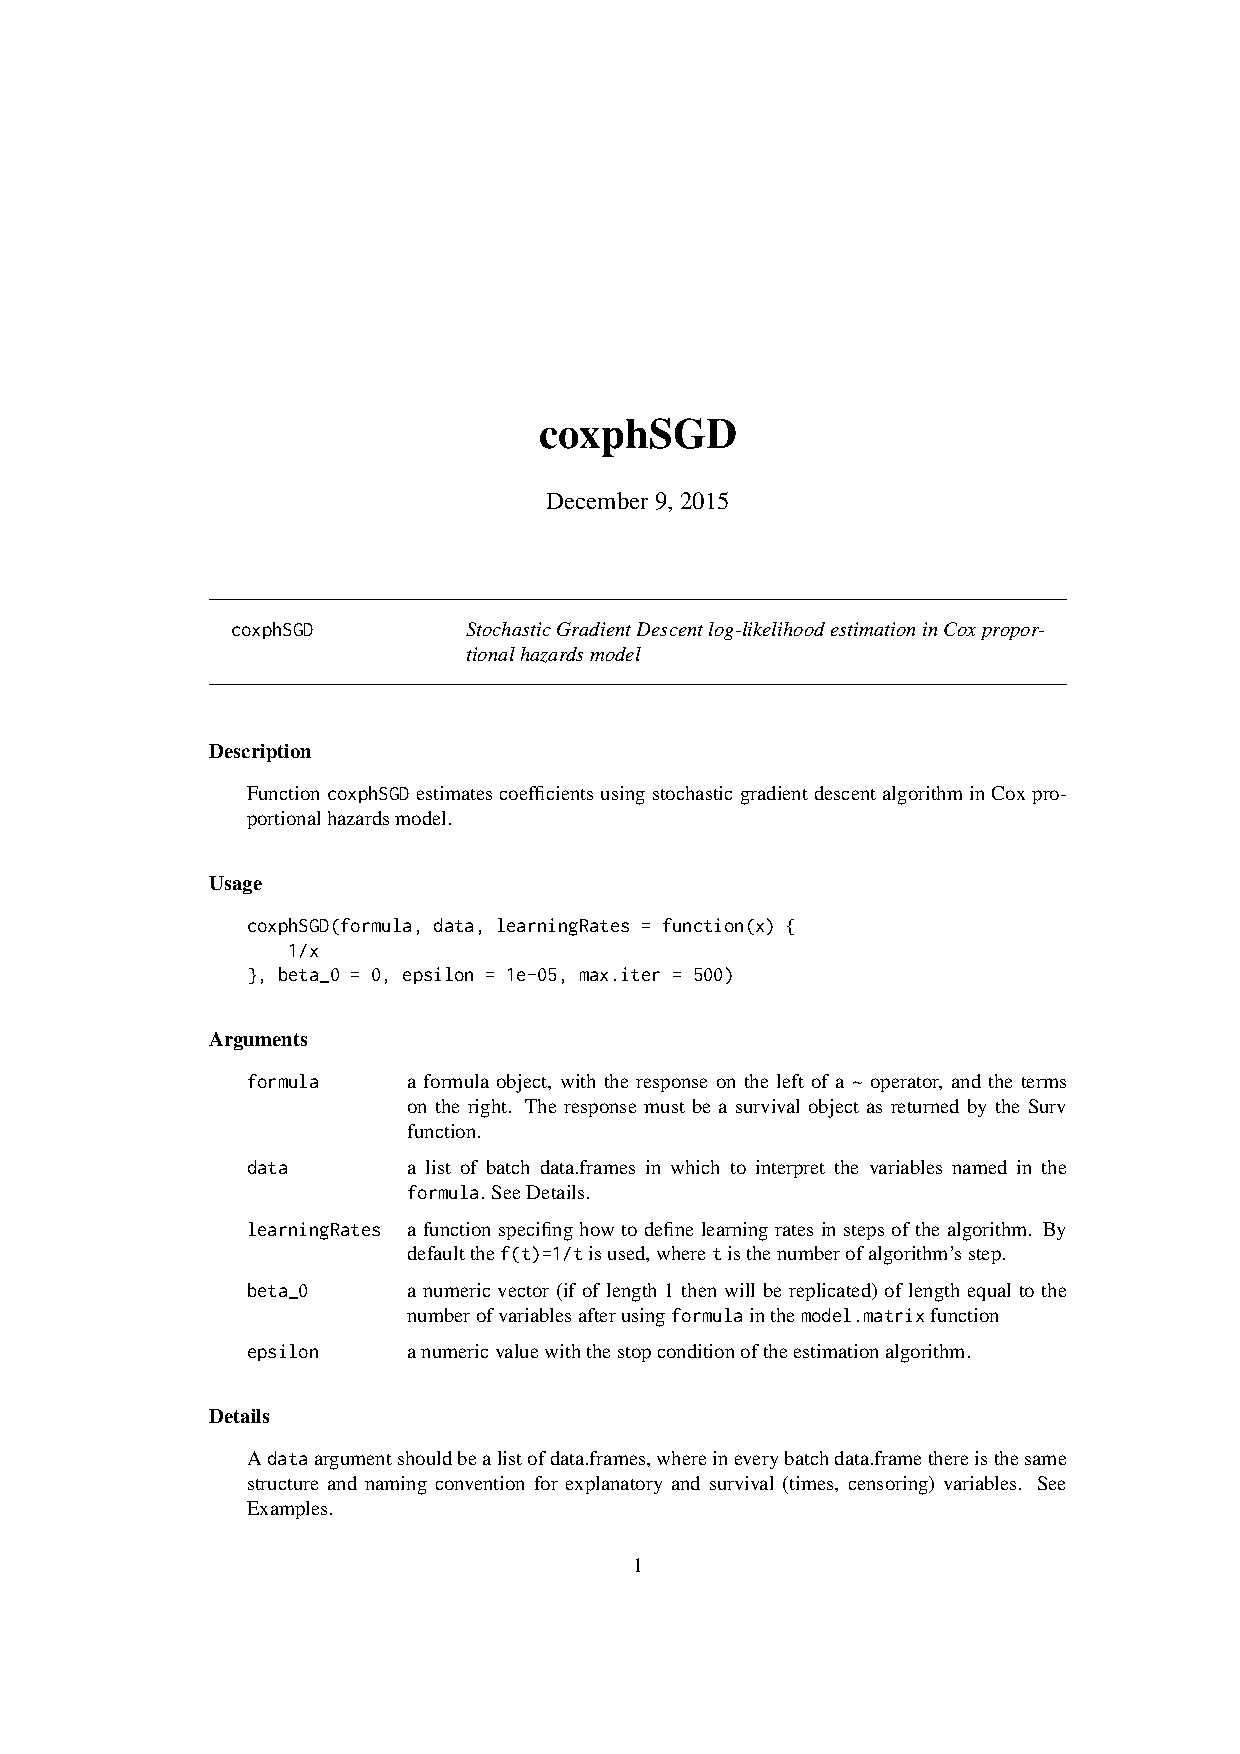
\includepdf[pages=-]{coxDoc8.pdf}
%\chapter{Dokumentacja pakietu RTCGA}
%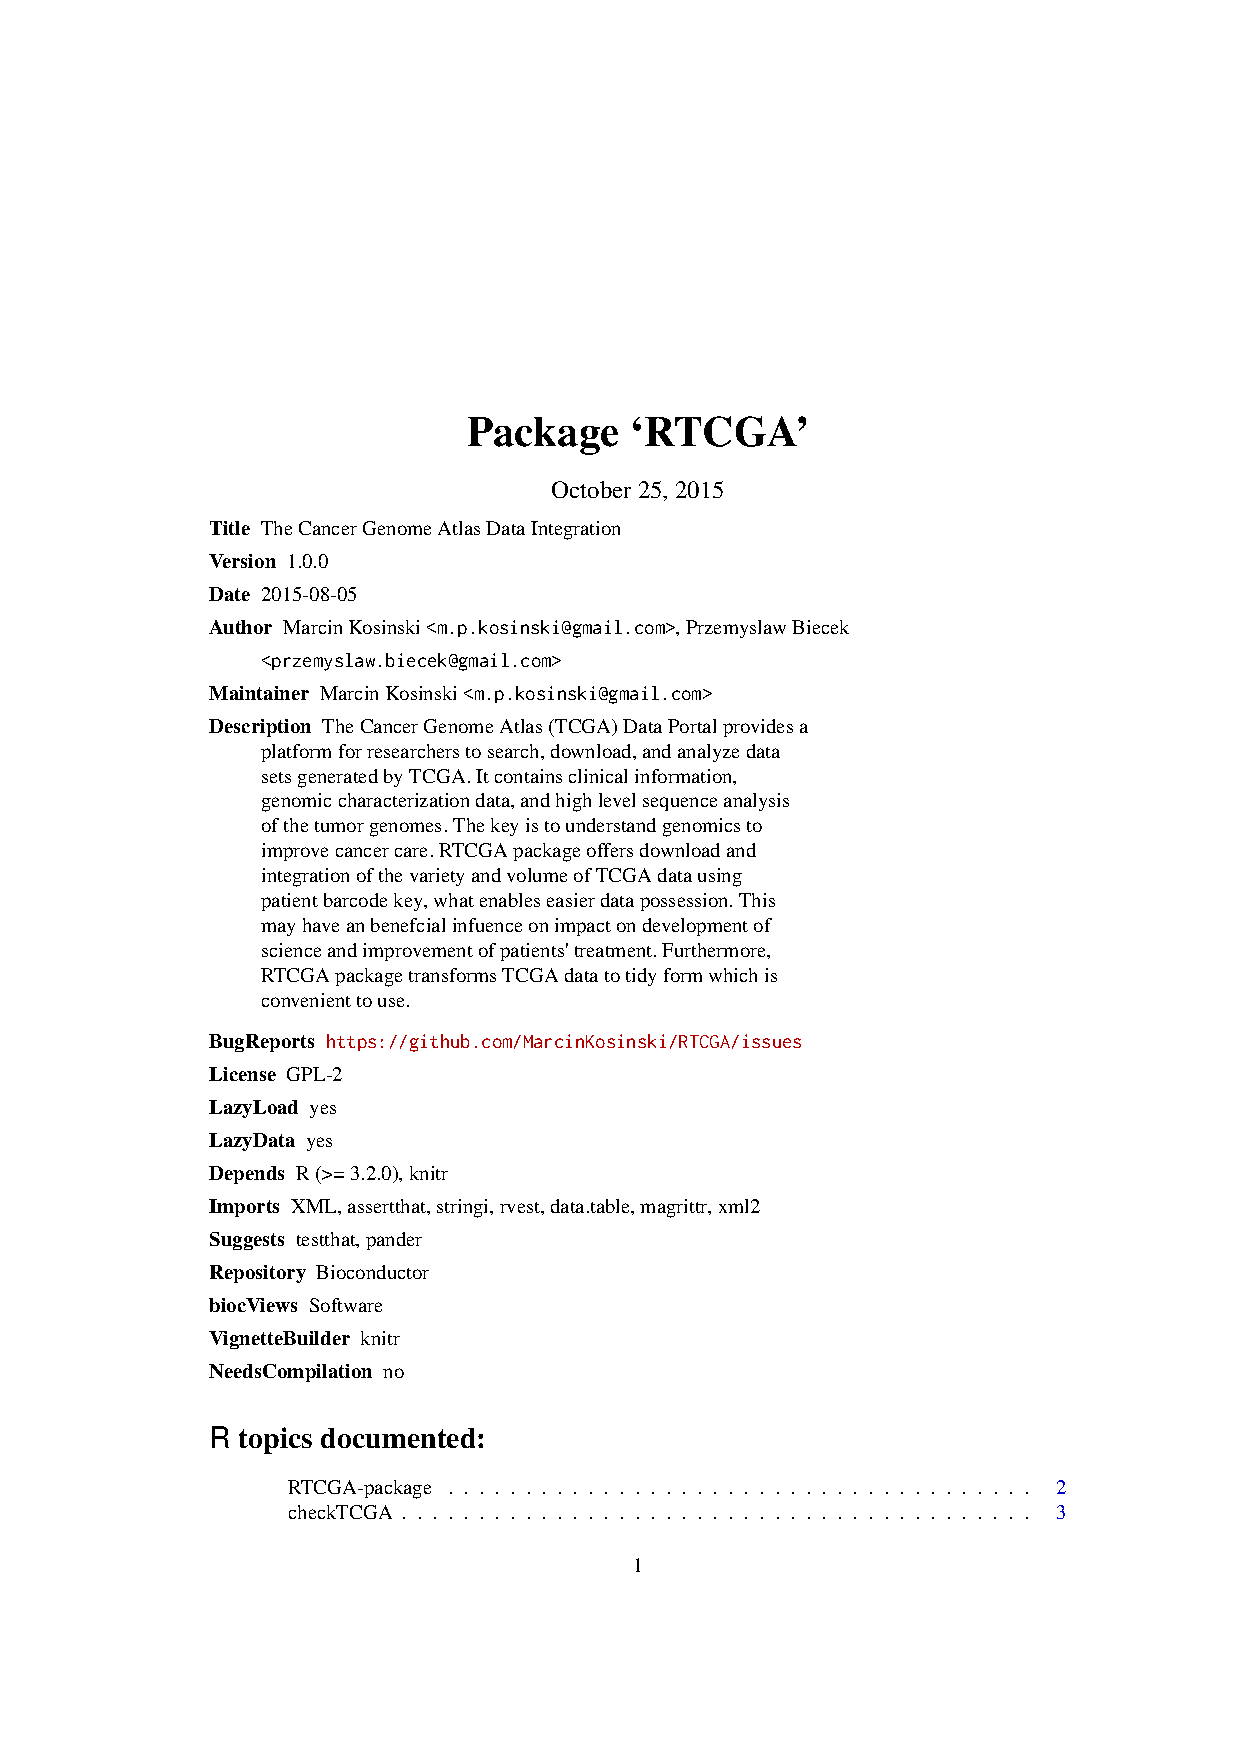
\includepdf[pages=-]{RTCGA.pdf}